\section{Using the cyclomatic complexity metric}

The cyclomatic complexity metric can be used to guide the development within the Kuadrant projects.
But it cannot be used as a metric that to be shown on some dashboard.
It is not even a metric that should be tracked overtime.
The two main usages I have seen do not require the tracking overtime.

\subsection{Guide for testing}
Reading many articles on \ccnsp, one of the use cases that I came across was using the metric for writing unit tests.
The idea is that you should write at least the same number of unit tests for a function as the \cc metric.
This metric will not cover all the possible iterations of a function or the edge case that need to be tested, but do give a good starting point.

To explore this concept, there is a sample function that gives time stamps a weight depending on when the time stamp is.
If we look at the function defined in \textbf{Figure \ref{fig:go_ex_1}} we can see that the \cc metric is 3, as there are two \textit{if statements} and a \textit{return statement}.
Currently, four unit tests would cover every possible outcome from that function.
The function makes a decision on weather the give timestamp is a weekend day and if the time is after noon.

\begin{figure}
	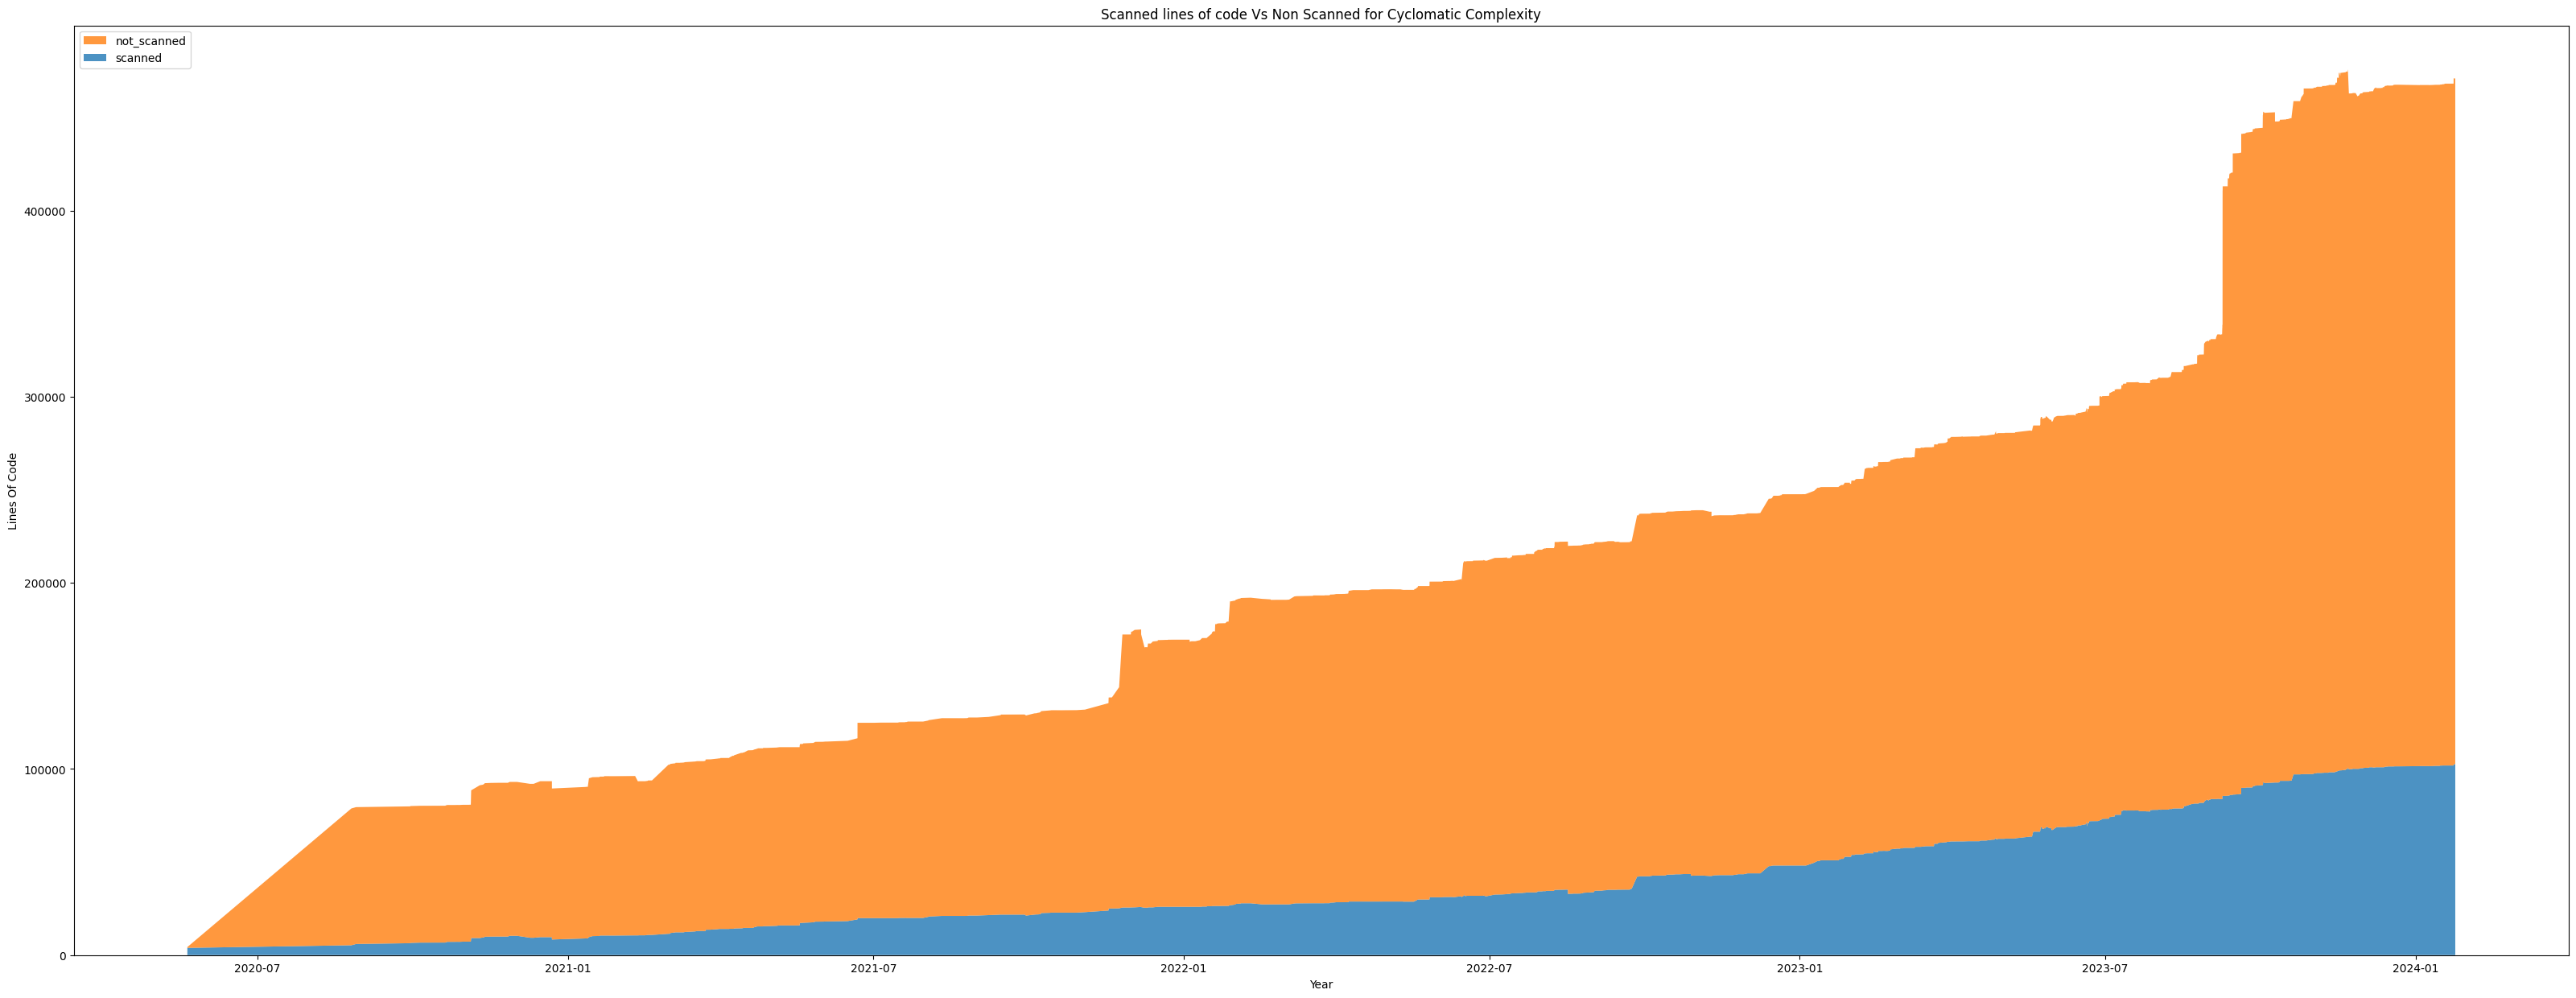
\includegraphics[width=\textwidth]{project_scanned_loc.png}
	\caption{Go function with a \cc of 3}
	\label{fig:go_ex_1}
\end{figure}

Let's make this code more complex, let's change the weighting base on if there is a \textit{"r"} in the days' name.
This change can be seen in \textbf{Figure \ref{fig:go_ex_2}}.
The interesting thing about this code is the \cc metric is now 4, but it requires eight unit tests to cover all possible outcomes of the function.
It shows that as the \cc metric goes up, the number of unit tests can explode.

\begin{figure}
	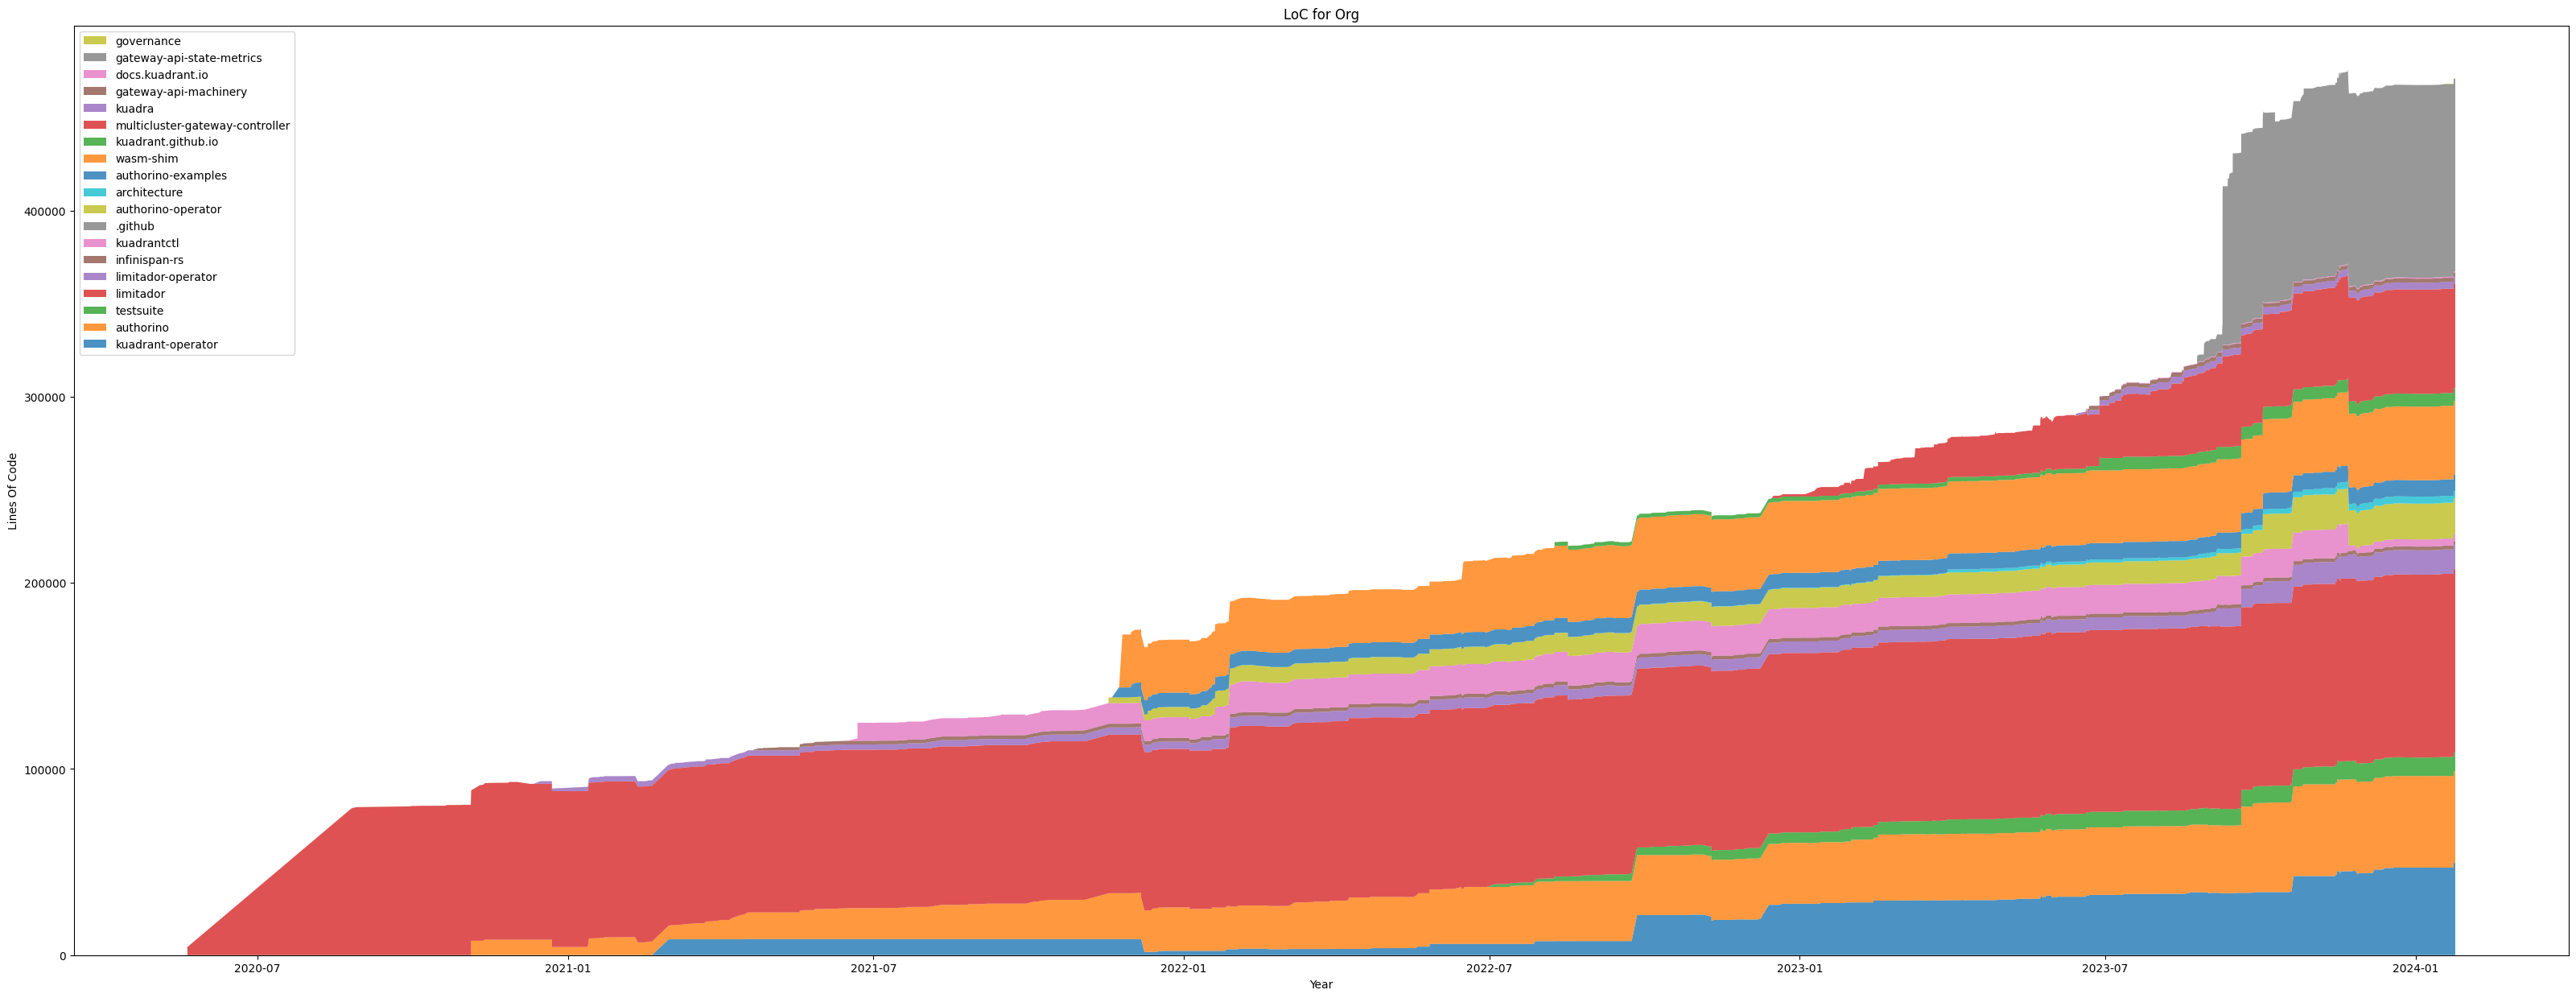
\includegraphics[width=\textwidth]{project_loc.png}
	\caption{Go function with a \cc of 4}
	\label{fig:go_ex_2}
\end{figure}

The other interesting thing about the function in \textbf{Figure \ref{fig:go_ex_2}} is how code coverage is affected.
You can achieve 100\% code coverage with using only two test cases.
This falls far below the testing all possible outcomes, but it makes the metric watchers happy.

So the \cc metric gives a developer of how many test cases they should be writing for a function to get a good coverage of the possible outcomes in the function.
While at the same time, not being crazy in the number of tests that is required.

\subsubsection{The 10\textsuperscript{th} September 1752 problem.}
I bring up this problem as it shows how the \cc metric cannot answer many questions a developer many need to be asking about their code.
On the 10\textsuperscript{th} September 1752 there are many places in the world that you could have been.
But you could not have been in most areas in Canada or the United States or the United Kingdom and its colonies because that date did not exist.
This was the time these places switched from the Julian Calendar to the Gregorian Calendar, a process that took 300 years around to complete\footnote{\href{https://www.timeanddate.com/calendar/julian-gregorian-switch.html}{Gregorian Calendar Reform: Why Are Some Dates Missing?}}.
With the last happening in Turkey at the start of 1927.

The example functions above many handle these dates but how can we be sure.
If this code needs to be location-aware and allow for times in the past, then these are edge cases that could happen.
The responsibility is still on the developer to know what should be tested.
No metric, not even \cc will help with identifying edge cases that need to be tested.

\subsection{Aiding system design}
Using \cc to aid in system design will depend somewhat on the school of though around what scores are acceptable.
If you are a follower of the \textit{"Clean Code"} teaching were functions should be short, then the \cc metric shows what functions need refactoring to lower their metric score.
But if you believe interfaces should be deep and not shallow, then the metric can show you functions that are really not doing much but require developers to know of their existing.

The tool used to calculate the \cc score in Ruby by default only showed results with a score of seven or higher.
It even went as far as to return a none zero result.
This shows the authors of the tooling were opinionated about what score functions should have.
An opinion that would align with the teachings in the \textit{Clean Code}.

My personal opinion is functions should try to be in Rank B (6–10 range).
This would greatly reduce the number of APIs that a developer would be required to learn.
Yes, there can be other ranked functions, and there should be.
A reconcile loop function should have many checks which drive the \cc score upward.
But the idea of having wrapper functions to reduce the \cc score of one function seems wrong.
















